%Template pembuatan proposal skripsi.
\documentclass{jtetiproposalskripsi}

%-----------------------------------------------------------------
%Disini awal masukan untuk data proposal skripsi
%---------- -------------------------------------------------------
\titleind{APLIKASI SISTEM ADMINISTRASI CUTI ONLINE
DI PT. PRUDENTIAL LIFE ASSURANCE
}

\fullname{Lintang Novitasari }

\idnum{1200631017}

\approvaldate{7 Januari 2015}

\degree{Sarjana Teknik }

\yearsubmit{2015}

\program{Menejemen informatika}
\headprogram{Bagus Setya,S.T.,M.T.,Ph.D.}

\firstsupervisor{Victor Wahanggara,S.Kom}
\firstnip{129 838 29 129}

\secondsupervisor{Triawan Adi Cahyanto, M.Kom}
\secondnip{12909 98009 5789}




%-----------------------------------------------------------------
%Disini akhir masukan untuk data proposal skripsi
%-----------------------------------------------------------------
\begin{document}

\cover
\approvalpage


%-----------------------------------------------------------------
%Disini akhir masukan untuk muka skripsi
%-----------------------------------------------------------------

%-----------------------------------------------------------------
%Disini awal masukan Intisari
%-----------------------------------------------------------------
\begin{abstractind}
Saat ini hampir semua kegiatan dikerjakan secara otomatis permasalahan yang terjadi adalah pada PT.Prudential masih menggunakan sistem perizinan cuti secara manual sehingga dalam penginputan data cuti sering terjadi kesalahan-kesalahan dan informasi yang dibutuhkan tidak dapat diperoleh secara cepat, akurat.Sebagai salah satu perusahaan asuransi,PT.Prudential memiliki standart cuti untuk karyawan  yang sejauh ini masih menggunakan sistem manual dengan membuat surat di kertas yang memiliki banyak sekali kekurangan.Kelemahan pada sistem lama adalah sistem cuti memerlukan validasi yang lama.Maka dari itu untuk menghindari hal tersebut kami membuat Sistem administrasi cuti onlain berbasis web.




\end{abstractind}
%-----------------------------------------------------------------
%Disini akhir masukan Intisari
%-----------------------------------------------------------------

\tableofcontents
\addcontentsline{toc}{chapter}{DAFTAR ISI}
\selectlanguage{bahasa}\clearpage\pagenumbering{arabic}\setcounter{page}{1}

%-----------------------------------------------------------------
%Disini awal masukan untuk Bab
%-----------------------------------------------------------------
\chapter{LATAR BELAKANG}

\section{Latar Belakang Masalah}
	Pertumbuhan dan perkembangan teknologi informasi saat ini semakin meningkat dengan pesat, Oleh karena itu tuntutan teknologi informasi pada suatu perusahaan merupakan suatu keharusan untuk diterapkan sebagai basis pengolahan data agar mampu mengikuti arus perkembangan informasi di era globalisasi. PT. Prudential Life Assurance (Prudential Indonesia) adalah perusahaan yang bergerak dibidang asuransi dengan cara seseorang mengikatkan diri kepada perusahaan agar mendapatkan perlindungan terhadap jiwa mereka dimasa yang akan datang. Menimbang peran fungsi teknologi informasi pada PT. Prudential Life Assurance sudah diterapkan manajemen administrasi didalam proses bisnisnya yaitu sistem administrasi yang menangani permasalahan perizinan cuti karyawan. Dimana perizinan cuti karyawan dianggap sebagai salah satu penunjang aset perusahaan terkait dengan kesejahteraan karyawan. Oleh karena itu manajemen pengolahan sistem administrasi cuti menjadi hal yang patut untuk dipertimbangkan dalam permasalahan di PT. Prudential Life Assurance.

Namun yang terjadi sistem administrasi perizinan cuti karyawan di PT. Prudential Life Assurance saat ini masih menggunakan sebuah pengajuan cuti mengggunakan formulir dokumen dimana manajemen perizinan ini terdapat kelemahan dan permasalahan. Permasalahan yang timbul dari sistem administrasi perizinan antara lain yaitu tentang respon validasi perizinan pimpinan yang membutuhkan waktu yang cukup lama dan sulitnya memanajemen kekosongan karyawan yang ada serta menentukan prioritas karyawan pada perusahaan yang diizinkan dan tidaknya akan mempengaruhi aktifitas kerja. 

Menanggapi permasalahan perizinan cuti pada PT. Prudential Life Assurance, solusi yang diharapkan yaitu membangun suatu sistem yang berfungsi sebagai pengolah data karyawan terkait dengan perizinan cuti. Dengan tujuan data perizinan karyawan tersimpan dalam media yang sudah disediakan untuk mengatasi terjadinya hilangnya dokumen atau duplikasi data sehingga akan memudahkan dalam proses memanajemen pengolahan data. 
Rencana sistem perizinan cuti yang akan dibuat menggunakan bahasa pemrograman PHP dan database MySQL. PHP adalah sebuah bahasa pemrograman yang biasanya dipasang pada dokumen HTML. Tujuan utama dari penggunan bahasa pemrograman PHP adalah untuk memungkinkan perancang web yang dinamis dan dapat bekerja secara otomatis. Sedangkan MySQL adalah sistem manajemen basisdata relasi yang bersifat terbuka atau open source yang digunakan untuk penyimpan data dalam mengembangkan aplikasi web.  
Sehubungan dengan alasan tersebut penulis bermaksud mencoba membuat sebuah aplikasi berbasis web denga judul PEMBUATAN APLIKASI SISTEM ADMINISTRASI CUTI ONLINE DI PT.PRUDENTIAL LIFE ASSURANCE.


\section{Rumusan  Masalah}
Dari permasalahan diatas maka didapatkan rumusan masalah sebagai berikut:
\begin{itemize}
\item[1.] Bagaimana merancang aplikasi sistem administrasi cuti online pada PT. Prudential Life Assurance?
\item[2.]Bagaimana membangun aplikasi sistem administrasi cuti online pada PT. Prudential Life Assurance?
\item[3.]Bagaimana menerapkan aplikasi sistem administrasi cuti online pada PT. Prudential Life Assurance?
\end{itemize}

\section{Batasan Masalah}
Agar permasalahan tidak menyimpang dari pembahasan maka dibuat batasan masalah sebagai berikut:
\begin{itemize}
\item[1.] Mengolah informasi tentang data pegawai yang cuti pada PT. Prudential Life Assurance.
\item[2.] Sistem yang akan dibangun menggunakan bahasa pemrograman PHP dan Pengolahan data MySql.
\item[3.] Pada sistem administrasi cuti memuat tentang input data pegawai cuti agar memperoleh laporan tentang kekosongan karyawan.
\end{itemize}

\section{Tujuan dan Manfaat Penelitian}	
\subsection{Tujuan Penelitian}
Adapun tujuan penelitian sebagai berikut:
\begin{itemize}
\item[1.]Merancang aplikasi sistem administrasi cuti online pada PT. Prudential Life Assurance.
\item[2.]Membangun aplikasi sistem adminnistrasi cuti online pada PT. Prudential Life Assurance.
\item[3.]Menerapkan aplikasi sistem administrasi cuti online pada PT. Prudential Life Assurance.

\end{itemize}
\subsection{Manfaat Penelitian}
Adapun manfaat penelitian adalah sebagai berikut:
\begin{itemize}
\item[1.]Untuk membantu proses cuti pada PT. Prudential Life Assurance.
\item[2.]Diharapkan sistem administrasi cuti online dapat membantu proses cuti agar tidak memakan waktu 			 lama dalam proses validasinya.
\end{itemize}




\chapter{LANDASAN TEORI}

\section{Tentang PT. Prudential Life Assurance}

	Didirikan pada tahun 1995, PT Prudential Life Assurance (Prudential Indonesia) merupakan bagian dari Prudential plc, sebuah grup perusahaan jasa keuangan terkemuka di Inggris. Sebagai bagian dari Grup yang berpengalaman lebih dari 165 tahun di industri asuransi jiwa, Prudential Indonesia memiliki komitmen untuk mengembangkan bisnisnya di Indonesia. Sejak meluncurkan produk asuransi yang dikaitkan dengan investasi (unit link) pertamanya di tahun 1999, Prudential Indonesia merupakan pemimpin pasar untuk produk tersebut di Indonesia. Di samping itu, Prudential Indonesia juga menyediakan berbagai produk yang dirancang untuk memenuhi dan melengkapi setiap kebutuhan para nasabahnya di Indonesia.	
Sampai 30 Juni 2014, Prudential Indonesia memiliki kantor pusat di Jakarta dan kantor pemasaran di Medan, Surabaya, Bandung, Denpasar, Batam dan Semarang. Prudential Indonesia melayani lebih dari 2,3 juta nasabah melalui lebih dari 200.000 tenaga pemasar di 371 Kantor Pemasaran Mandiri (KPM) di seluruh nusantara (termasuk di Jakarta, Surabaya, Medan, Bandung, Yogyakarta, Batam, dan Bali).
\section{Sistem Administrasi}

	Sistem Administrasi  adalah usaha dan kegiatan yang berkenaan dengan penyelenggaraan kebijaksanaan untuk mencapai tujuan.Administrasi dalam arti sempit adalah kegiatan yang meliputi: catat-mencatat, surat-menyurat, pembukuan ringan, ketik-mengetik, agenda, dan sebagainya yang bersifat teknis ketatausahaan.Administrasi dalam arti luas adalah seluruh proses kerja sama antara dua orang atau lebih dalam mencapai tujuan dengan memanfaatkan sarana prasarana tertentu secara berdaya guna dan berhasil guna.
\section{Perizinan Cuti}
Perizinan cuti adalah keadaan tidak masuk kerja yang diizinkan dalam jangka waktu terntu .
Macam-macam perusahaan
\begin{itemize}
\item[1.] Cuti Tahunan
\item[2.] Cuti Sakit
\item[3.] Cuti Bersalin
\item[4.]	Cuti karena alasan penting
\end{itemize}

\section{PHP} 
	PHP sendiri sebenarnya merupakan singkatan dari “Hypertext Preprocessor”, yang merupakan sebuah bahasa scripting tingkat tinggi yang dipasang pada dokumen HTML. Sebagian besar sintaks dalam PHP mirip dengan bahasa C, Java dan Perl, namun pada PHP ada beberapa fungsi yang lebih  spesifik. Sedangkan tujuan utama dari penggunaan bahasa ini adalah untuk memungkinkan perancang web yang dinamis dan dapat bekerja secara otomatis.
 
Gambar 2.1 Bagan Cara kerja PHP
PHP merupakan Server Side Scripting, dimana PHP selalumembutuhkan web server dalam menjalankan aksinya. Secara prinsip, server akan bekerja apabila ada permintaan dari client, yaitu kode – kode PHP . Client tersebut akan dikirimkan kepada server, kemudian server akan mengembalikan pada halaman sesuai instruksi yang diminta. Inilah cara kerja PHP:
\begin{itemize}
\item 	Server membaca permintaan dari client/browser.
\item 	Server membaca permintaan dari client/browser.
\item 	Kemudian dilanjutkan untuk mencari halaman / page server.
\item 	Server melakukan instruksi yang diberikan oleh PHP untuk melakukan modifikasi pada halamanpage.
\item 	Selanjutnya hasil modifikasi tersebut akan dikembalikan kepada client atau browser
\end{itemize}

\section{Sejarah PHP
 	PHP dibuat pertama kali ole}h Rasmus Lerdorf, yang pada awalnya dibuat untuk menghitung jumlah pengunjung pada home pagenya. Awalnya PHP kependekan dari personal home page saat itu namanya masih Form Interpreted. Selanjutnya pembuat PHP merilis kode sumber (open source) ke khalayak umum sehingga banyak programmer yang tertarik untuk mengembangkan PHP. (Virgi, 2011: 10-11)
\subsection{Kelebihan dan Kekurangan PHP}
Kelebihan PHP
\begin{itemize}
\item[1.]Bahasa pemrograman PHP adalah sebuah bahasa script yang tidak melakukan sebuah kompilasi dalam 			 penggunaanya.
\item[2.]Web Server yang mendukung PHP dapat ditemukan dimana - mana dari mulai apache, IIS, Lighttpd, 		         hingga Xitami dengan konfigurasi yang relatif mudah.
\item[3.]Dalam sisi pengembangan lebih mudah, karena banyaknya milis -  milis dan developer yang siap 			     membantu dalam pengembangan.
\item[4.]Dalam sisi pemahaman, PHP adalah bahasa scripting yang paling mudah karena memiliki referensi 	   	     yang banyak.
\item[5.]PHP adalah bahasa open source yang dapat digunakan diberbagai mesin (Linux, Unix, Macintosh, 	  			 Windows) dan dapat dijalankan secara runtime melalui console serta juga dapat menjalankan 	  			     perintah-perintah system.
\end{itemize} 
	
Kelemahan PHP :
\begin{itemize}
\item[1.]Tidak ideal untuk pengembangan skala besar
\item[2.]Tidak memiliki sistem pemrograman berorientasi objek yang sesungguhnya (sampai versi 4 ini)
\item[3.]Tidak bisa memisahkan antara tampilan dengan logik dengan baik (walau penggunaan template dapat 			 memperbaikinya)
\item[4.]PHP memiliki kelemahan security tertentu apabila programmer tidak jeli dalam melakukan 		  	         pemrograman dan kurang memperhatikan isu dan konfigurasi PHP
\item[6.]Kode PHP dapat dibaca semua orang, dan kompilasi hanya dapat dilakukan dengan tool yang mahal 	   	     dari Zend.
\end{itemize}

\section{XAMPP}
			XAMPP adalah perangkat lunak bebas yang mendukung banyak sistem operasi yang merupakan kompilasi dari beberapa program. Fungsinya adalah sebagai server yang berdiri sendiri (localhost), yang terdiri atas program Apache HTTP Server, MySQL database dan penerjemah bahasa yang ditulis dengan bahasa pemrograman PHP dan Perl.
Nama XAMPP merupakan singkatan dari X (empat sistem operasi apapun), Apache, MySQL, PHP dan Perl. Program ini tersedia dalam General Public License (GNU) dan bebas, merupakan web server yang mudah digunakan yang dapat melayani tampilan halaman web yang dinamis.  

XAMPP adalah kepanjangan yang masing-masing hurufnya adalah:

X 	:Program ini dapat dijalankan dibanyak sistem operasi, seperti Windows, Linux, Mac OS, danjuga 			 	 Solaris.

A 	:Apache, merupakan aplikasi web server. Tugas utama Apache adalah menghasilkan halaman web yang benar 		 kepada user berdasarkan kode PHP yang dituliskan oleh pembuat web, maka dapat saja suatu database 		 	 diakses terlebih dahulu (misalnya dalam MySQL) untuk mendukung halaman web yang dihasilkan.

M 	:MySQL, merupakan aplikasi database server. Perkembangannya disebut SQL yang merupakan kepanjangan 		 	 dari Structure Query Language. SQL merupakan bahasa terstruktur yang digunakan untuk mengolah 			     database. 

	 MySQL dapat digunakan untuk membuat dan mengelola database besertaisinya. Kita dapat memanfaatkan 			 MySQL untuk menambahkan, mengubah dan menghapus data yang berada dalam database.
	 
P 	:PHP, bahasa pemrograman web. Bahasa pemrograman PHP merupakan bahasa pemrograman untuk membuat web 		 yang bersifat server-side scripting. PHP memungkinkan kita untuk membuat halaman web yang bersifat 		 dinamis. Sistem manajemen basis data yang sering digunakan bersama PHP adalah MySQL.

P 	:Perl adalah bahasa pemrograman untuk segala keperluan, dikembangkan pertama kali oleh Larry Wall di 		 mesin Unix. Perl dirilis pertama kali pada tanggal 18 Desember 1987 ditandai dengan keluarnya Perl 1.
	 Pada versi-versi selanjutnya, Perl tersedia pula untuk berbagai sistem operasi varian Unix (SunOS, 		 Linux, BSD, HP-UX), juga tersedia untuk sistem operasi seperti DOS, Windows, Power PC, BeOS, VMS, 			 EBCDIC, dan PocketPC. (Rachmad Hakim, 2010: 120-121)
	 
\section{Tools Perancangan Sistem}
\subsection{Flowchart Sistem}
Menurut  Raymond Jr McLeod menyatakan bahwa System flowchart merupakan bagan yang menunjukkan arus pekerjaan secara keseluruhan dari sistem. Bagan ini menjelaskan urut – urutan dari prosedur – prosedur yang ada di dalam sistem. Flowchart menunjukkan apa yang dikerjakan di sistem. Simbol – simbol yang digunakan dalam system flowchart adalah sebagai berikut :

\subsection{Flowchart Sistem}
 \begin{figure}[ht!]
  \centering
    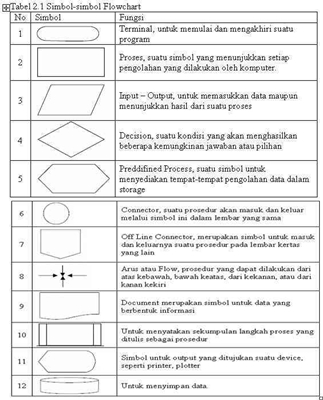
\includegraphics{gambar/lin}
    \caption{Simbol Flowchartsistem}
    \label{lin}
\end{figure}


\subsection{Data Flow Diagram (DFD)}
		Data Flow Diagram (DFD) adalah suatu gambaran grafis dari suatu sistem yang menggunakan sejumlah bentuk-bentuk simbol untuk menggambarkan bagaimana data mengalir melalui suatu proses yang saling berkaitan (McLeod,1996).
		DFD sering digunakan untuk menggambarkan suatu sistem yang telah ada atau sistem baru yang akan dikembangkan secara logika tanpa mempertimbangkan lingkungan fisik dimana data tersebut mengalir(misalnya lewat telepon,surat dan sebagainya)atau lingkungan fisik dimana data tersebut akan disimpan (misalnya file kartu,harddisk,tape,diskette,dan sebagainya). DFD merupakan alat yang digunakan pada metodologi pengembangan sistem yang terstruktur. DFDmerupakan alat  yang cukup populer sekarang ini ,karena dapat menggambarkan arus data di dalam sistem dengan terstruktur.

\subsection{Simbol DFD}
 \begin{figure}[ht!]
  \centering
    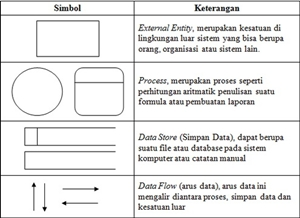
\includegraphics{gambar/cew}
    \caption{Simbol DFD}
    \label{cew}
\end{figure}



\subsection{ Entity Relationship Diagram (ERD)}
	Model Entity-Relationship berisi komponen-komponen dari suatu himpunan entitas dan himpunan relasi yang masing-masing dilengkapi dengan atribut-atribut yang merepresentasikan seluruh fakta yang ditinjau sehingga dapat diketahui hubungan antara entity-entity yang ada dengan atribut-atributnya. Selain itu juga  ias menggambarkan hubungan yang ada dalam pengolahan data, seperti hubungan many to many, one to many, atau one to one. Lebih jelasnya akan digambarkan secara sistematis dengan menggunakan Diagram Entity-Relationship (Diagram E-R / ERD).
Simbol-simbol yang digunakan dalam Entity Relationship Diagram dijelaskan pada gambar berikut ini :

\subsection{Simbol ERD}
 \begin{figure}[ht!]
  \centering
    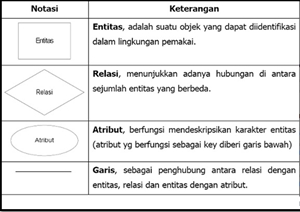
\includegraphics{gambar/erd}
    \caption{Simbol ERD}
    \label{erd}
\end{figure}




Hubungan/relasi antar atribut yang terdapat pada sistem konseptual secara bebas yang terdiri dari entity-entity, dan setiap entiti terdiri dari atribut yang ada, yaitu :
\begin{itemize}
\item[1.]Unary, adalah satu entiti berelasi  hanya dengan satu entiti saja.
\item[2.]Binary, adalah satu entiti berhubungan dengan entiti yang lain.
\item[3.]Ternary, adalah satu entiti berhubungan dengan beberapa entiti yang lainnya. 
\end{itemize}
	 
\section{Database}

Database adalah sistem penyimpanan beragam jenis data dalam sebuah entitas yang besar untuk diolah sedemikian rupa agar mudah dipergunakan lagi. Data yang disimpan bisa sangat variatif (angka, teks, gambar, suara, dan jenis data multi-media lainnya). Basis data merupakan kumpulan dari data yang saling berhubungan satu dengan yang lainnya, tersimpan di perangkat keras computer dan digunakan perangkat lunak untuk memanipulasinya. Database merupakan salah satu komponen yang penting dalam sistem informasi,karena merupakan basis dalam menyediakan informasi bagi para pemakai. (Sucipto, 2012: 137).

MySQL merupakan sebuah basis data yang mengandung satu atau beberapa kolom. Tabel terdiri atas sejumlah basis dan setiap baris mengandung satu atau beberapa kolom. Didalam PHP telah menyediakan fungsi untuk koneksi ke basis data dengan sejumlah fungsi untuk pengaturan baik menghubungkan maupun memutuskan koneksi server database MySQL sebagai sarana untuk mengumpulkan informasi. (Yeni Kustiyahningsih, Devie Rosa Anamisa, 2010: 145-146).

MySQL adalah sistem manajemen basisdata relasi yang bersifat terbuka atau open source. Sistem manajemen basisdata ini adalah hasil pemikiran dari Michael “Monty” Widenius, David Axmark, dan Allan Larson pada tahun 1995. Tujuan awal ditulisnya program MySQL adalah untuk mengembangkan aplikasi web. MySQL menggunakan bahasa standar SQL (Structure Query Language) sebagai bahasa interaktif dalam mengelola data. 
Perintah SQL sering juga disebut Query. MySQL menawarkan berbagai keunggulan dibandingkan database server lain.
Berikut ini adalah beberapa keunggulan MySQL:
\begin{itemize}
\item[1.]Mampu menangani jutaan user dalam waktu yang bersamaan.
\item[2.]	Mampu menampung lebih dari 50.000.000 record.
\item[3.]	Sangat cepat mengeksekusi perintah.
\item[4.]	Memiliki user privilege system yang mudah dan efisien.
\end{itemize} 
Kelemahan MySQL:
\begin{itemize}
\item[1.]Untuk koneksi ke bahasa pemrograman visual seperti vb, delphi, dan foxpro, mysql kurang support, 			 karena koneksi ini menyebabkan field yang dibaca harus sesuai dengan koneksi dari program visual 	   		 tersebut, dan ini yang menyebabkan mysql jarang dipakai dalam program visual.
\item[2.]Data yang ditangani belum begitu besar.
\end{itemize}
	
\subsection{CDM} 	
          Conceptual Data Model (CDM) merupakan salah satu bentuk dari hubungan antar entitas atau Entity Relationship Diagram (ERD). Namun yang membedakan adalah Conceptual Data Model (CDM) dibuat dengan menggunakan sebuah software Power Designer.Power Designer adalah software yang digunakan untuk pembuatan perancangan tabel Entity Relationship Diagram (ERD) yaitu Conceptual Data Model (CDM) dan Physical Data Model (PDM).
\subsection{PDM}	
Physical Data Model (PDM) merupakan hasil dari proses generate dari Conceptual Data Model (CDM) yang sudah dibuat Apabila CDM yang dibuat masih terdapat error (maksud dari ERROR disini adalah missal: Relasi yang kurang benar dan nama field tidak boleh sama pada karakternya) maka Physical Data Model (PDM) tidak bisa dibuat.




\chapter{METODOLOGI PENELITIAN}

\section{Metode Penelitian}
Metode penelitian sangat penting untuk menyusun Aplikasi sistem cuti online karena sangat erat hubungannya dengan prosedur,teknik dan desain penelitian yang akan dirancang. Didalam metode penelitian ini terdapat beberapa tahap,tahapan-tahapan tersebut adalah:
\subsection{Study Literatur}
Study literatur dilakukan untuk mengetahui dan mengkaji secara teoritis,metode yang dipakai untuk memecahkan masalh yaitu dengan cara mencari data-data yang berhubungan dengan sistem parking.
\subsection{Pengumpulan data}
Penulis menggunakan beberapa teknik pengumpulan data sebagai berikut:
\begin{itemize}
\item[1.]Observasi
Observasi yaitu teknik pengumpulan data dengan mengadakan pengamatan
dan pencatatan mengenai kegiatan-kegiatan yang dilakukan oleh bagian
administrasi, dengan maksud untuk memudahkan dalam penyusunan  laporan tugas akhir.
\item[2.]Interview
Interview yaitu teknik pengumpulan data dengan meminta keterangan dari
pihak-pihak yang berwenang untuk memberikan keterangan tentang data yang
dibutuhkan agar data menjadi lebih lengkap dan jelas.
\item[3.]Dokumentasi
Dokumentasi yaitu teknik pengumpulan data dengan cara mengumpulkan
data, laporan atau tulisan dari bagian yang berhubungan dengan data cuti.
\end{itemize}

\subsection{Analisis sistem} 

Analisis sistem adalah penguraian dari suatu sistem informasi yang utuh kedalam bagian-bagian komponennya dengan maksud untuk mengidentifikasikan dan mengevaluasi permasalahan,kesempatan, hambatan yang terjadi dan kebutuhan yang diharapkan sehingga dapat diusulkan perbaikan.Kegiatan-kegiatan dalam analisis sistem dapat dilihat dibawah ini.
\begin{itemize}
\item[a.]Memahami kinerja sistem, pada langkah ini diperlukan hal-hal sebagai berikut.
\item[1.]Memahami kerja dari sistem yang digunakan
\item[2.]Mengatur jadwal penelitian
\item[b.]Menganalisa sistem, hal-hal yang perlu dianalisis.
\item[1.]Menganalisis kelemahan sistem
\item[2.]Menganalisis kebutuhan informasi atau manajemen
\end{itemize}
\subsection{Optimasi Data}
\begin{itemize}
\item[a.] Model Prosedural:Model yang bersifat deskriptif sesuai dengan prosedur yang telah ditentukan.
\item[b.] Model Konseptual:Model yang menggariskan langkah-langkah yang harus diikuti untuk menghasilkan 			  sistem yang baik.
\end{itemize}

\subsection{Perancangan sistem} 
Perancangan sistem yang baik diperlukan untuk pembuatan program yang baik tak terkecuali dalam pembuatan sistem informasi yang baik. Perancangan sistem secara terperinci, dilakukan dengan cara sebagai berikut.
\begin{itemize}
\item[1.]Perancangan sistem informasi
		 Merancang sistem informasi yang akan dibuat dan dilanjutkan dengan perancangan database.
\item[2.]Pembangunan database
\end{itemize}

Tahap-tahap dari pembuatan database
\subsection{Implementasi}
Implementasi sistem merupakan tahap untuk merealisasikan hasildesain/perancangan sistem yang telah dilakukan sebelumnya kedalam bentuk yang sebenarnya. Tahap implementasi sistem terdiri dari langkah-langkah sebagai berikut:

\begin{itemize}
\item[a.]Menerapkan Rencana Implementasi
		 Rencana implementasi dimaksudkan untuk mengatur biaya dan waktu yang dibutuhkan selama tahap 			  	 implementasi sistem. 
\item[b.]Melakukan Kegiatan Implementasi
		 Kegiatan-kegiatan yang dilakukan dalam tahap implementasi ini adalah sebagai berikut:
\item[1.]Pemograman (Coding Program)
		 Pemograman (Coding Program) adalah kegiatan menulis kode program yang akan dieksekusi oleh 				komputer. Kode program yang ditulis oleh pemrogram harus berdasarkan dokumentasi yang disediakan oleh analis sistem hasil dari desain sistem secara rinci. Hasil program yang sesuai dengan desain, akan menghasilkan program yang dibutuhkan oleh pemakai sistem.
\item[2.] Pengetesan Program (Testing Program)
Pengetesan Program (Testing Program) adalah kegiatan untuk mengetahui kesalahan-kesalahan yang mungkin terjadi dalam pembuatan program. Kesalahan dari program yang mungkin terjadi dapat diklasifikasikan dalam tiga bentuk kesalahan .
\item[A.]Kesalahan bahasa (language errors)
		 Kesalahan bahasa adalah kesalahan didalam penulisan source program yang tidaksesuai dengan yang 			 disyaratkan.
\item[B.]Kesalahan sewaktu proses (run time errors)
		 Kesalahan sewaktu proses adalah kesalahan yang terjadi sewaktu-waktu. executable program 					 dijalankan. Kesalahan ini akan menyebabkan proses program berhenti sebelum selesai pada saatnya, 		     karena kompiler menemukankondisi-kondisi yang belum terpenuhi sehingga tidak bisa dikerjakan.
\item[C.]Kesalahan logika (logical errors)
		 Kesalahan logika adalah kesalahan dari logika program yang dibuat.Kesalahanseperti ini sulit 				 ditemukan, karena tidak ada pemberitahuan mengenai kesalahan dan tetap didapatkan hasil dari 					proses program, tetapi hasilnya salah.
\item[D.]Pengetesan Sistem
		 Pengetesan sistem dilakukan untuk memeriksa kekompakan antar komponen sistem yang diimplementasi. 		 Tujuan utama dari pengetesan sistem ini adalah untuk memastikan bahwa elemen-elemen atau 					 komponen-komponen dari sistem telah berfungsi sesuai dengan yang diharapkan. Pengetesan perlu 				 dilakukan untuk mencari kesalahan-kesalahan atau kelemahan-kelemahan yang mungkin masih terjadi.

\end{itemize}

\subsection{Pelaporan}
Proses dan hasil penelitian yang telah diperoleh dituangkan dalam bentuk laporan.
\section{Desain Sistem}
Untuk Menganalisa masalah dari pemakai atau sasaran dari aplikasi ini maka dibuatlah suatu desain sistem dan juga desain sistem merupakan gambaran ,perencanaan dan pembuatan dengan menyatukan masalah yang terpisah ke dalam satu kesatuan yang utuh untuk memperjelas bentuk sebuah sistem. Tahapan-tahapan dalam desain sistem tersebut yaitu:

\subsection{Flowchart Sistem}
 \begin{figure}[ht!]
  \centering
    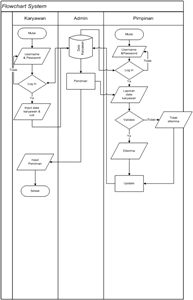
\includegraphics{gambar/flow}
    \caption{Flowchartsistem}
    \label{flow}
\end{figure}
  
Keterangan:
\begin{itemize}
\item[1.]Mulai
\item[2.]Username dan Password karyawan diperoleh dari database karyawan
\item[3.]Karyawan melakukan Login,jika validasinya YA maka ke proses selanjutnya yaitu input data karyawan 		 dan cuti, jika TIDAK maka kembali ke Uasername dan password.
\item[4.]Jika sudah mengisi Input data karyawan dan cuti maka data akan tersimpan di database.
\item[5.]Username dan Password Pimpinan diperoleh dari database karyawan
\item[6.]Pimpinan melakukan Login,jika validasinya YA maka ke proses selanjutnya yaitu mendapat laporan 			 dari admin tentang data karyawan dan cuti, jika TIDAK maka kembali ke Username dan password.
\item[7.]Pimpinan melakukan Validasi,Jika YA maka cuti diterima akan terupdate datanya,Jika TIDAK maka  			 cuti tidak diterima akan terupdate.
\item[8.]Proses update akan masuk ke dalam database.
\item[9.]	Admin memproses perizinan
\item[10.]	Karyawan menerima Hasil Perizinan cuti
\item[11.]	Selesai
\end{itemize}

\section{Alat Bantu}

Untuk kelancaran dalam penelitian ini, berikut penjelasan mengenai alat bantu yang penulis gunakan, yaitu : 
\subsection{Perangkat Keras (Hardware)}
Perangkat Keras (Hardware) yang digunakan dalam pembuatan perancangan  sistem ini adalah satu unit Laptop     dengan spesifikasi sebagai berikut : 
\begin{itemize}
\item[a.] Processor : Intel ® Core ® CPU 
               P6200 @ 2.40 Ghz 
\item[b.] Memori : 2 GB DDR3 Memory 
\item[c.] Hardisk : 32 GB HDD 
\end{itemize}

\subsection{Perangkat Lunak} 
 untuk mempermudah software yang digunakan dalam penyusunan Aplikasi ini antara lain : 
 \begin{itemize}
\item[a.] Microsoft Office Word 2010 
\item[b.] Microsoft Office Visio 2007 
\item[c.] NotePad++
\item[d.] PowerDesaingner 15.0
 \end{itemize}



\section{Pengujian}
Proses pengujian dapat dilakukan setelah aplikasi yang kita buat telah selesai.Tujuan pengujian adalah untuk memastikan aplikasi yang kita buat benar-benar bisa digunakan atau belum bisa digunakan.

\section{ Jadwal Penelitian}


\vspace{-0.5cm}
\begin{figure}[ht!]
  \centering
    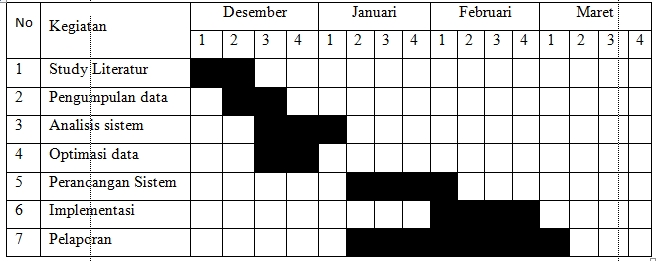
\includegraphics[width=13cm]{gambar/jadwal}
    \begin{center}
Tabel 3.1. Jadwal Penelitian.
\end{center}
\end{figure}




%-------------------------------------------------------------------------------












%-----------------------------------------------------------------
%Disini akhir masukan Bab
%-----------------------------------------------------------------

%-----------------------------------------------------------------
%Disini awal masukan untuk Daftar Pustaka
%-----------------------------------------------------------------
%%\nocite{Abel2010,Guerbas201350}
%%\bibliography{research-plan}
%%\bibliographystyle{plainnat}
\begin{thebibliography}{9}

\bibitem[satu(2013)]{satu01}
Spinar, R., dkk, ``Demo Abstract: Efficient Building Management with IP- based Wireless Sensor Network'', , 6th European Conference on Wireless Sensor Networks. Cork, Ireland 11-13 February 2009.

\bibitem[dua(2013)]{dua02}
Adam Dunkels, Thiemo Voigt, Niclas Bergman, dan Mats Jonsson ``The Design and Implementation of an IP-based Sensor Network for Intrusion Monitoring'', Swedish National Computer Networking Workshop, Sweden, 2004.

\bibitem[tiga(2013)]{tiga03}
Sigit B. Wibowo, dan Widyawan, ``Wireless Sensor Network and Internet Protocol Integration with COTS'', 2013 AUN/SEED-Net Regional Conference in Electrical and Electronics Engineering, Bangkok, Thailand, 2013.

\bibitem[empat(2013)]{empat04}
Dokumen online, http://www.iqrf.org/, IQRF, diakses pada Maret 2013

\bibitem[lima(2013)]{lima05}
Widyawan, Sigit B. Wibowo, dkk, ``iHome: Low-Cost Domotic for Residential Houses'', 5th AUN/SEED-Net Regional Conference on Information and Communications Technology (RCICT), Manila, Filipina, 2012.

\bibitem[enam(2013)]{enam06}
Dokumen online,https://openwrt.org/, diakses pada Maret 2013

\bibitem[tujuh(2013)]{tujuh07}
Dokumen online, http://www.digi.com/technology/rf-articles/wireless-zigbe,
diakses pada Maret 2013.

\end{thebibliography}
\addcontentsline{toc}{chapter}{DAFTAR PUSTAKA}
%-----------------------------------------------------------------
%Disini akhir masukan Daftar Pustaka
%-----------------------------------------------------------------

\end{document}